\documentclass{../acm_proc_article-me11_tweaked}
\usepackage[usenames,dvipsnames,svgnames,table]{xcolor}
\usepackage{graphicx}
\usepackage{url}
\usepackage{caption}
\DeclareCaptionType{copyrightbox}
\usepackage{subcaption}

\begin{document}

\conferenceinfo{\textit{MediaEval 2013 Workshop,}}{October 18-19, 2013, Barcelona, Spain}

\title{Identifying the Geographic Location of an Image with a Multimodal Probability Density Function}

%
\def\sharedaffiliation{%
\end{tabular}
\begin{tabular}{c}}
%

\numberofauthors{8}
\author{
\alignauthor
Jamie Davies\\
    \email{jagd1g11@ecs.soton.ac.uk}
\and
\alignauthor
Jonathon S. Hare\\
    \email{jsh2@ecs.soton.ac.uk}
\and
\alignauthor
Sina Samangooei\\
    \email{ss@ecs.soton.ac.uk}
\and
\alignauthor
John Preston\\
    \email{jlp1g11@ecs.soton.ac.uk}
\and
\alignauthor
Neha Jain\\
    \email{nj1g12@ecs.soton.ac.uk}
\and
\alignauthor
David P. Dupplaw
    \email{dpd@ecs.soton.ac.uk}
\sharedaffiliation
    \affaddr{Electronics and Computer Science, University of Southampton, United Kingdom}
}

\additionalauthors{Additional author: Paul H. Lewis (email: {\texttt{phl@ecs.soton.ac.uk}})}

\maketitle
\begin{abstract}
% Knowing the location that a photograph was taken provides us with data that could be useful in a wide spectrum of applications. With the advance of digital cameras, and with many users exchanging their digital cameras for their GPS-enabled mobile phones, photographs annotated with geographical locations are becoming ever more present on photo-sharing websites such as Flickr. However there is still a wide majority of online content that is not geotagged, meaning that algorithms for efficient and accurate geographical estimation of an image are needed. We present a general model for using both textual metadata and visual features of photos to automatically place them on a world map.
There is a wide array of online photographic content that is not geotagged. Algorithms for efficient and accurate geographical estimation of an image are needed to geolocate these photos. This paper presents a general model for using both textual metadata and visual features of photos to automatically place them on a world map.
\end{abstract}

%\keywords{Geotagging, Probability Density, Image Annotation}

\section{Introduction and Motivation}
The primary goal of the 2013 MediaEval placing task~\cite{mediaevalPlacing13} was to develop techniques for accurately predicting the geo-location of a set of Flickr images in terms of latitude and longitude. In addition, a secondary goal was to enhance predictions by estimating the error of the predicted location of each image. The task organisers provided a set of approximately 8.5 million images with metadata and locations for training, and a set of 262,000 images without geotags for testing.

The motivation for the techniques we have developed for the task was twofold; we firstly wanted to develop a technique that can operate using either the visual content or the metadata, but which also seamlessly allowed blending of information across modalities and allowed information from external gazetteers to be incorporated. Secondly, we wanted our technique to be scalable and efficient, with the aim of being able to estimate the position of an image in well under a second using standard desktop hardware.

\section{Overall Methodology}\label{sec:meth}
The basic idea of our approach is that we estimate a continuous probability density function (PDF) over the surface of the Earth from a number of \emph{features} extracted from the query image and/or its metadata. To estimate the PDF, each feature provides a fixed size set of \emph{points} (latitude, longitude) which are then combined, and a kernel density estimator can be used to estimate the probability density at any arbitrary position. By finding the modes of the PDF we create an estimate of the location of the photograph from the position of the mode with the highest probability. By fitting a univariate Gaussian over the support of the highest probability mode, we can estimate the accuracy of the estimated geolocation as a function of the variance.

% \begin{figure}
% 	\centering
% 	\begin{subfigure}[b]{0.48\columnwidth}
% 		\centering
% 		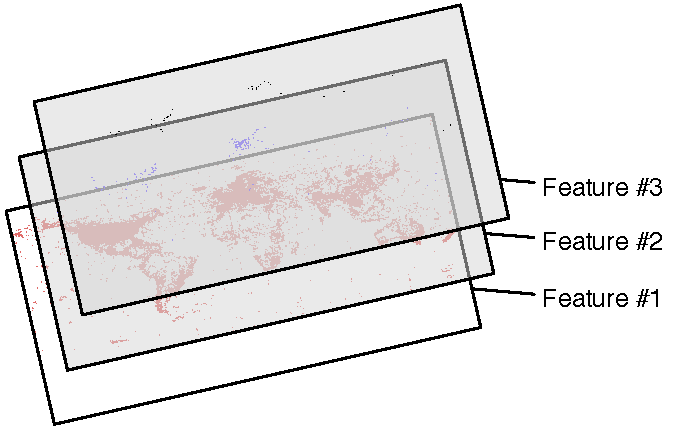
\includegraphics[width=\columnwidth]{images/layers}
% 		\caption{}
% 		\label{fig:features}
% 	\end{subfigure}
% 	~
% 	\begin{subfigure}[b]{0.48\columnwidth}
% 		\centering
% 		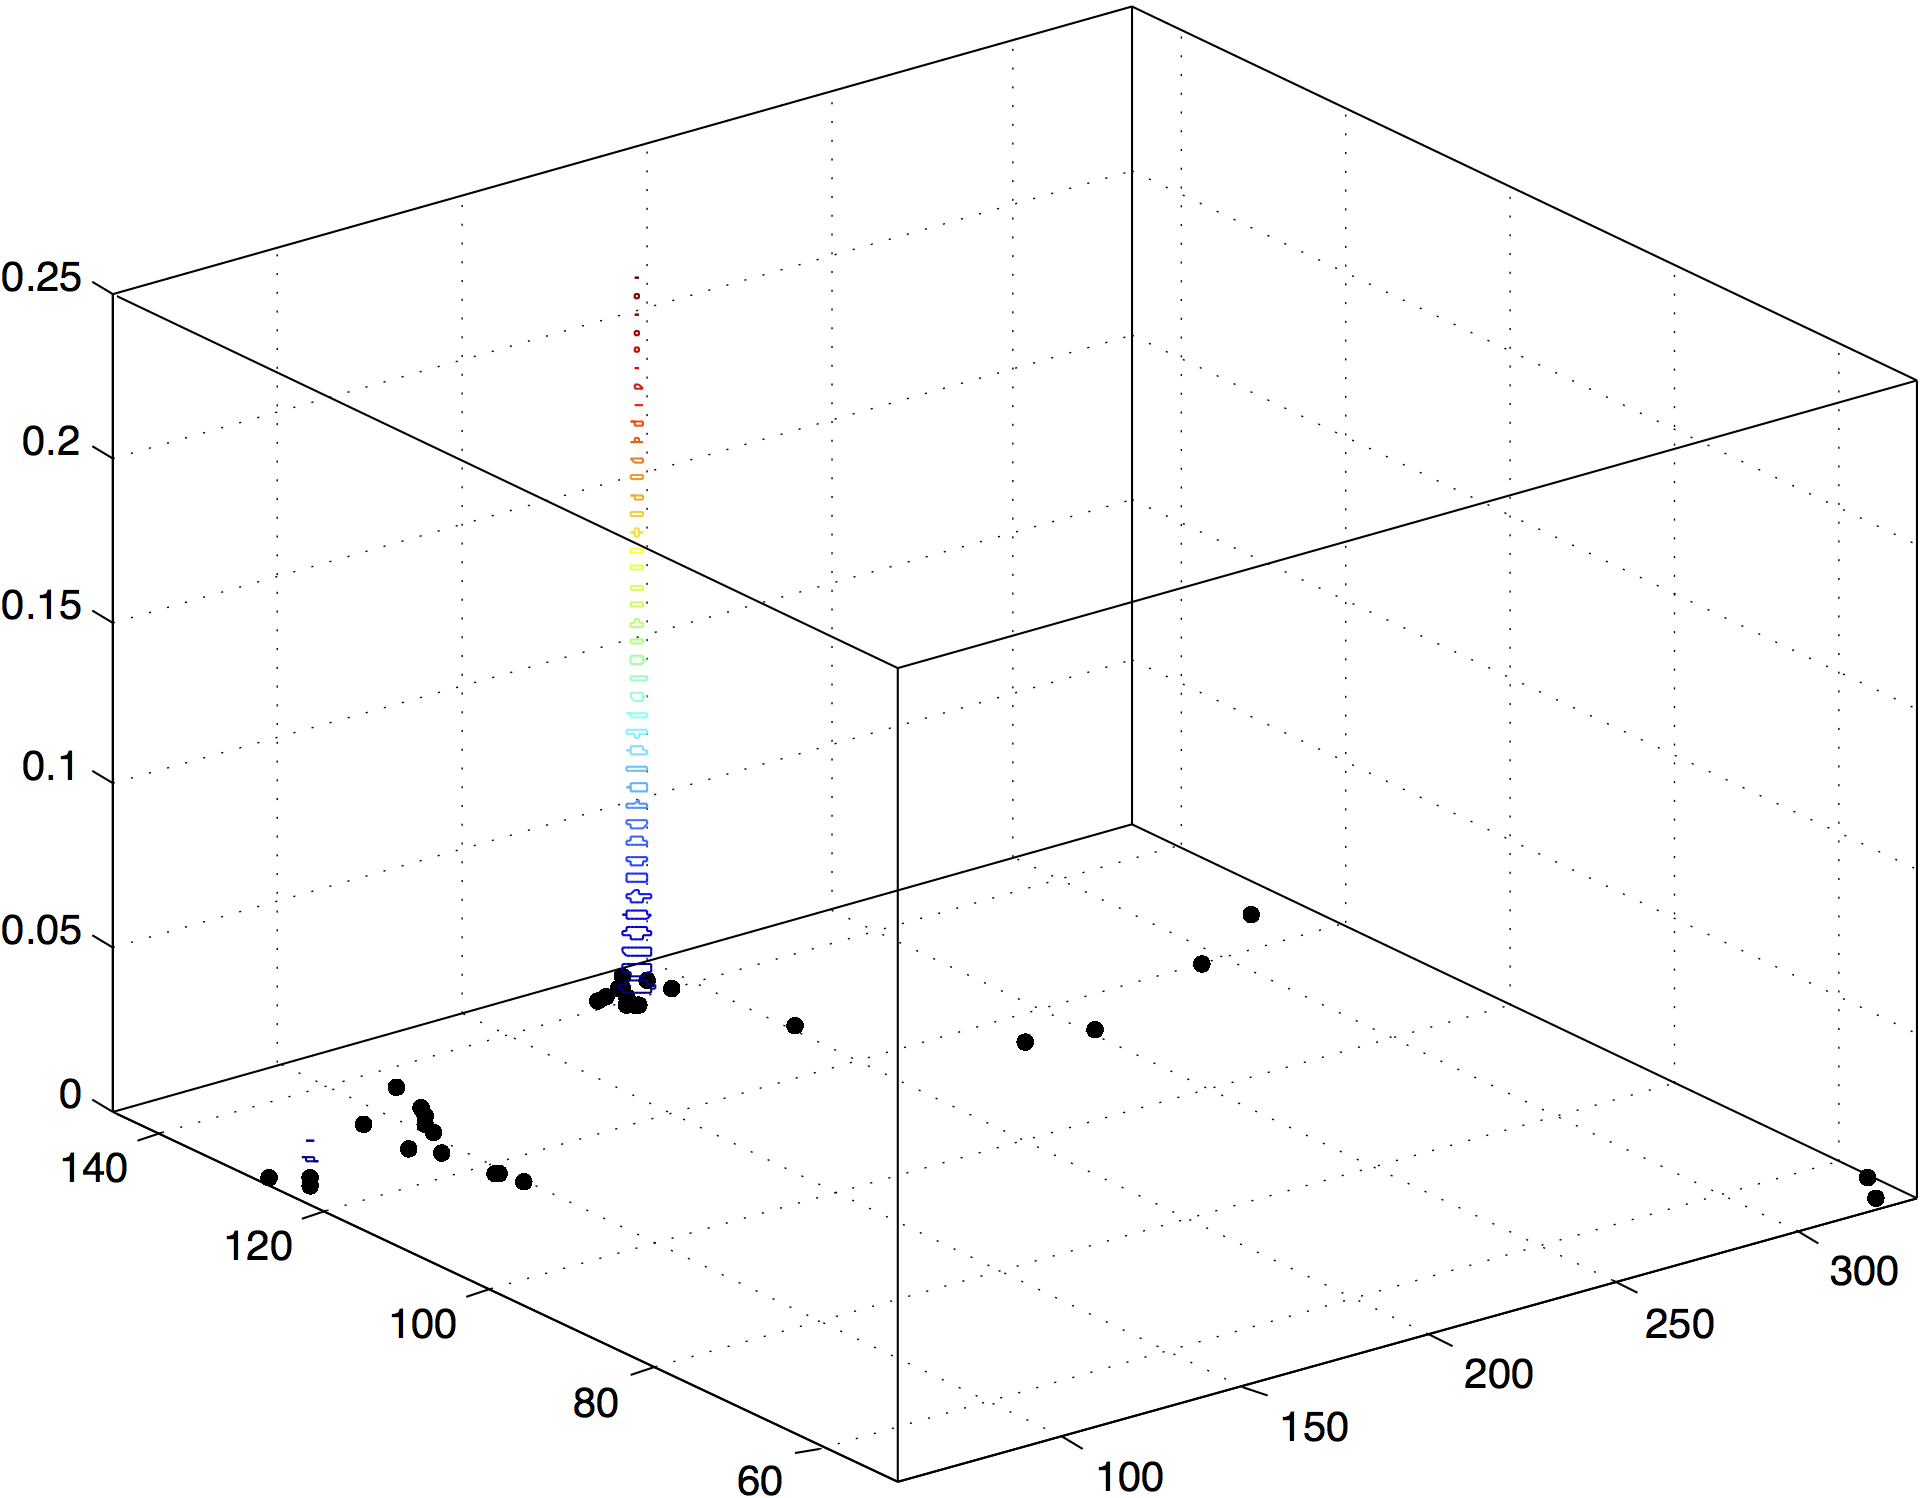
\includegraphics[width=0.8\columnwidth]{images/density}
% 		\caption{}
% 		\label{fig:density}
% 	\end{subfigure}
% 	\caption{(a) Sets of points representing the probability density of each feature are overlaid. (b) A kernel density estimator is applied and we estimate the photograph's location at the position of the largest peak in the density function.}
% \end{figure}

In practice, density estimation and mode-finding can be combined by applying the mean-shift algorithm. Mean-shift has been used in the context of geolocation estimation in the past; for example, Hays and Efros~\cite{Hays:2008:im2gps} used mean-shift on the results of content-based image search to determine probable locations. Our approach differs from that of Hays and Efros's, because, whereas they only considered single (high recall/low precision) content-based features, we consider the fusion of multiple features from different modalities. In addition, Hays and Efros used the mean-shift algorithm for coarse-grained location estimation, with a very large kernel bandwidth, whilst in our technique, because of the way we are using features we are able to use a much smaller kernel bandwidth for fine-grained location estimation.

\begin{table*}[ht!]
	\centering
	\caption{\label{tab:results}Results of the five runs}
	\begin{tabular}{|r||c|c|c|c|c|}
		\hline
		 & Run 1 & Run 2 & Run 3 & Run 4 & Run 5 \\ \hline \hline
		No. est. within 1km & 53449 (20.55\%) & 891 (0.34\%) & 60190 (23.15\%) & 68050 (26.17\%) & 61631 (23.70\%) \\ \hline
		No. est. within 10km & 81988 (31.53\%) & 1453 (0.56\%) & 98032 (37.70\%) & 106370 (40.9\%) & 100009 (38.47\%) \\ \hline
		No. est. within 100km & 93838 (36.09\%) & 2711 (0.10\%) & 113937 (43.82\%) & 123233 (47.40\%) & 114986 (44.23\%) \\ \hline
		No. est. within 500km & 10911741.97\% & 9174 (3.52\%) & 132655 (51.02\%) & 139136 (53.51\%) & 129721 (49.89\%) \\ \hline
		No. est. within 1000km & 122752 (47.21\%) & 19129 (7.36\%) & 147443 (56.71\%) & 151876 (58.41\%) & 141767 (54.53\%) \\ \hline
		Median error in km & 1352.897154 & 6898.266561 & 451.8928271 & 254.4838372 & 540.109773 \\ \hline
		Linear correlation of error & 0.1568 & 0.0594 & 0.3693 & 0.3721 & 0.0406 \\ \hline
	\end{tabular}
\end{table*}

\section{Experiments}
The implementation of our methodology was realised in Java using OpenIMAJ\footnote{\url{http://openimaj.org}}~\cite{Hare:2011:OIJ:2072298.2072421} and Lucene\footnote{\url{http://lucene.apache.org}}. For speed, we used an approximate mean-shift implementation inspired by the one in scikit-learn\footnote{\url{http://scikit-learn.org/stable/modules/clustering.html#mean-shift}}. The approximations stem from using a regular grid for determining the seed points from which to seek modes (rather than using the actual data), and using nearest-neighbours to assign data points to modes, rather than actually assigning them to the mode they converge to. A KD-Tree is used for efficient nearest neighbour lookup.

\subsection{Features}
The following features were used in our experiments. Each feature provides a set of geographic points in response to a query image:

\noindent\textbf{Location Prior}. A constant prior feature built by sampling 1000 geographical coordinates from the training data.

\noindent\textbf{Tags}. Every tag in the query image is associated with the coordinates of the training images in which the tag appeared. If a tag in the query was unseen in the training data, then it contributes no points. Each tag is considered to be an independent feature. No filtering of tags was performed.

\noindent\textbf{PQ-CEDD}. In order to provide a high-recall/low-precision image search we indexed the provided CEDD features with a product quantiser (18 products of 256 clusters) to enable fast in-memory search of the complete training data using the asymmetric distance computation method~\cite{Jegou:2011:PQN:1916487.1916695}. The locations of the 100 top images to a query formed the point set returned by the feature.

\noindent\textbf{LSH-SIFT}. High-precision (low recall) image content search was performed using a variant of the approach we developed in~~\cite{Hare:2013:TVP:2461466.2461514}. DoG-SIFT features were extracted from the images and hashed using Locality Sensitive Hashing. A graph was built with the images as the nodes, and edge weights were based on the number of collisions. In order to perform a query, the directly connected nodes to the query were detected in the graph, and their geo-coordinates returned.

\subsection{Runs}
For all of our submitted runs, the methodology described in Section~\ref{sec:meth} was applied. In all runs we used a flat kernel with bandwidth of $0.01^\circ$. All runs except for run \#5 used a constant number of 1000 points per feature (effectively making all features have a fixed weight); any feature that produced more or less points was randomly and uniformly sub- or super-sampled to reach 1000 points. In total, 5 runs were submitted. The configurations are summarised in Table~\ref{tab:runconf}. Notes about each run are listed below:


\begin{table}
    \centering
    \caption{The feature configuration for the run submissions.}
    \label{tab:runconf}
    % \begin{tabular}[h]{|l||*{5}{>{\centering\arraybackslash}m{1.3cm}|}}
    \begin{tabular}[h]{|l||c|c|c|c|}
        \hline
        % \multicolumn{1}{|c||}{} & \multicolumn{1}{c|}{\rothead[Prior]} & \multicolumn{1}{c|}{\rothead[Tags]} & \multicolumn{1}{c|}{\rothead[CEDD]} & \multicolumn{1}{c|}{\rothead[SIFT-LSH]}} \\
			  & Prior & Tags & PQ-CEDD & SIFT-LSH \\
        \hline        \hline
        Run 1 & \checkmark & \checkmark & \checkmark & \checkmark \\
        \hline
        Run 2 & \checkmark & & \checkmark & \checkmark \\
        \hline
        Run 3 & \checkmark & \checkmark & & \\
        \hline
        Run 4 & \checkmark & \checkmark & & \checkmark \\
        \hline
        Run 5 & \checkmark & \checkmark & \checkmark & \checkmark \\
        \hline
    \end{tabular}
\end{table}

\noindent\textbf{Runs 1-3: Provided data.}	The first three runs used features extracted from the provided dataset only. No external data was used.

\noindent\textbf{Run 4: Text+Visual, bigger dataset}. The fourth run used features extracted from a larger dataset of approximately 46 million geotagged Flickr images we collected last year. As with the provided data, only images with an accuracy of 16 were crawled. For the purposes of fair experimentation, we removed all photos from the users who appeared in the test set.

\noindent\textbf{Run 5: Text+Visual, provided data with tag boosting}. The fifth run was the same as run 1, but we used the GeoNames\footnote{http://www.geonames.org} gazetteer to boost the weight of tag features that were likely to belong to a specific geographic location; any textual tag that could be matched against the the GeoNames ``name'' or ``alternate-name'' field was boosted by doubling its number of points from 1000 to 2000. Non textual features, and tags that didn't match remained at 1000 points/feature.

\subsection{Results, Discussion and Future Work}
Our results are shown in Table~\ref{tab:results}. The first thing to note is that visual features alone perform relatively poorly for exactly predicting locations; this is be be expected as the vast majority of images do not contain recognisable places. Interestingly our first and fourth runs (text and visual) performed worse than the third (text only). This was unexpected and warrants further investigation as our experiments had indicated that the visual features should help boost performance. Run 4 indicates that using additional data helps our approach. We'd expect our error estimation to improve (higher correlation coefficient) as we become more accurate; this trend can be seen to an extent, although run 5 is a definite outlier. 
We had started to experiment with product-quantised PCA VLAD encodings of SIFT features, temporal features and query expansion of LSH-SIFT features, however we ran out of time to optimise and include these in the runs. It will be interesting to investigate these further, together with other features such as GIST in the future. It would also be interesting to try some other approaches to incorporating structured knowledge from GeoNames.

\section{Acknowledgments}
The described work was funded by the European Union Seventh Framework Programme (FP7/2007-2013) under grant agreements 270239 (ARCOMEM), and 287863 (TrendMiner).


\bibliographystyle{abbrv}
\bibliography{../bibliography}
\end{document}
